\documentclass{article} \usepackage{CJK}
\usepackage{CJK}
\usepackage{ctex}
\usepackage{graphicx}
\usepackage{float}
\graphicspath{{pic/}}
\renewcommand{\contentsname}{目录}
\renewcommand{\abstractname}{摘要}
\author{杨铭 - 5130379022\\
        李晟 - 5130379017\\
        张云翔 - 5130379012}
\title{HCI 课程选题提交\\\textbf{Cubeat}}
\begin{document}
\maketitle
\tableofcontents
\newpage
\section{Cubeat —— 项目简述}
\paragraph{手势+节拍}
\paragraph{}Cubeat是一款基于LeapMotion的音乐节拍游戏。通过LeapMotion对玩家的手部动作进行追踪,完成玩家在游戏内“魔方”上的各种操作,契合音乐节拍。
\begin{figure}[!h]
\begin{minipage}{0.5\linewidth}
  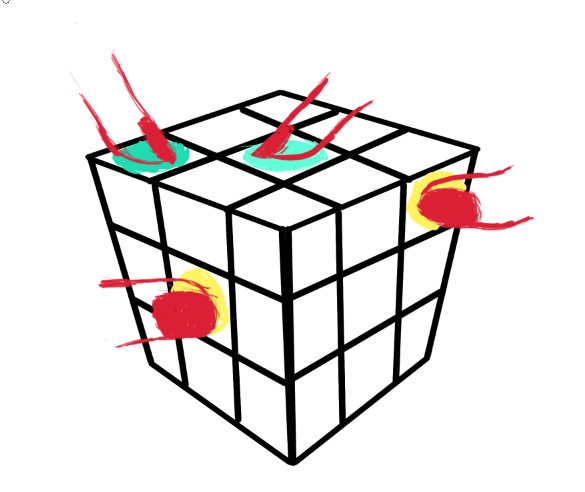
\includegraphics[width=18em]{pic1.png}\\
  \caption{}\label{1-1}
\end{minipage}
\begin{minipage}{0.5\linewidth}
  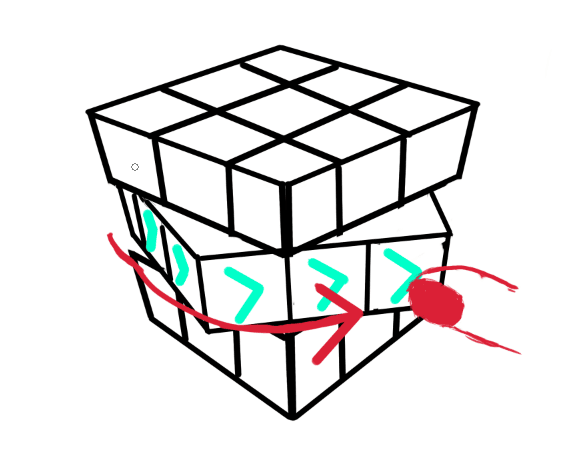
\includegraphics[width=18em]{pic2.png}\\
  \caption{}\label{1-2}
\end{minipage}
\end{figure}
\paragraph{}
本款产品作为一款音乐游戏,力图突破传统音游的游戏方式,使用最新的交互技术LeapMotion,给玩家提供最新潮的玩法。
\paragraph{}
由于LeapMotion的限制,Cubeat将是一款PC音乐游戏。
\newpage
\section{用户分析和需求}
\subsection{用户分析}
\paragraph{}
为了调查市场,我们组制作了一份调查问卷,主要针对青少年和大学生群体进行了调查。
\paragraph{对音乐游戏的熟悉程度}
\begin{figure}[h]
  \centering
  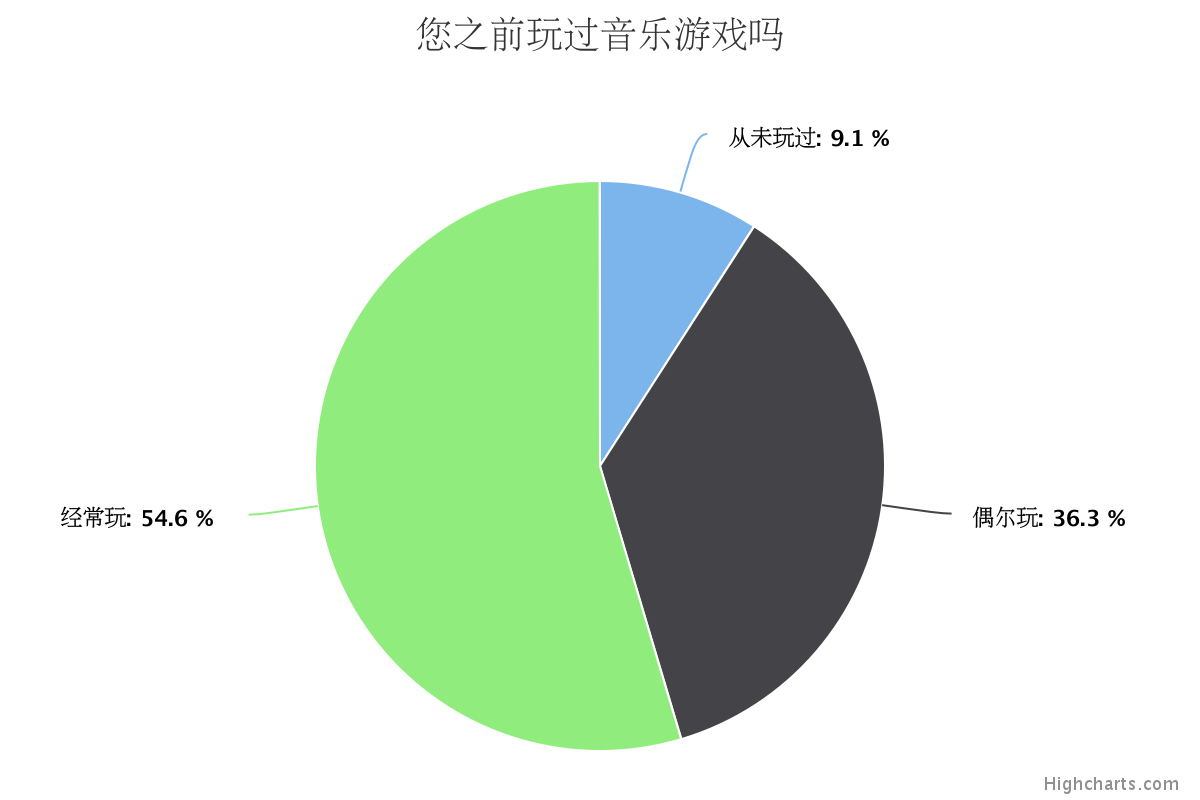
\includegraphics[width=25em]{chart1.png}\\
  \caption{您之前玩过音乐游戏吗}\label{2-1}
\end{figure}
\paragraph{}
由于在调查时,一些人表示不熟悉音乐游戏而拒绝了填写问卷,并且调查时间较短,所以推测数据有一定偏差。但从目前的数据来看,大多青少年和大学生都
玩过音乐游戏,一大半的人经常玩音乐游戏,可以看出音乐游戏的市场还是较为广阔。
\paragraph{玩音乐游戏的平台}
\begin{figure}[H]
  \centering
  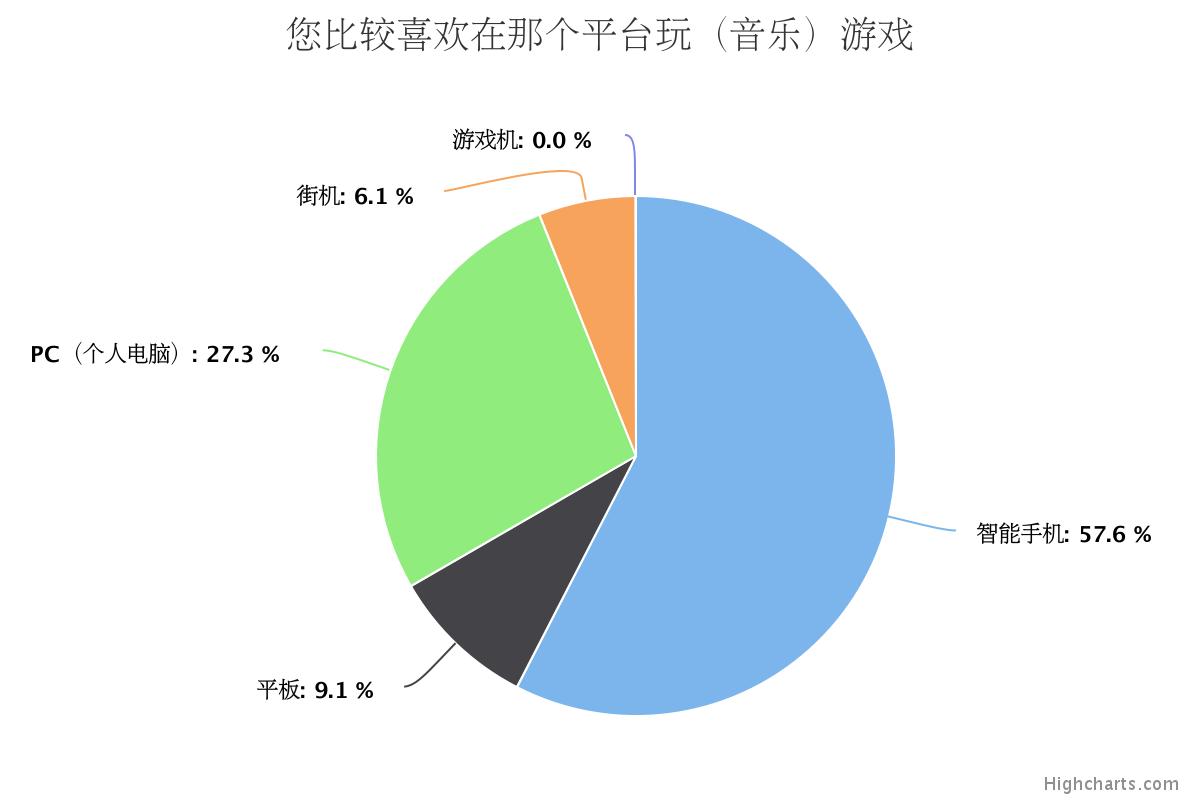
\includegraphics[width=22em]{chart2.png}\\
  \caption{您一般在那个平台玩(音乐)游戏}\label{2-2}
\end{figure}
\paragraph{}
随着智能手机的兴起,大家的娱乐时间日渐碎片化,从调查结果中也可见一斑。现在也有许多音乐游戏厂商在向智能手机或平板等移动设备进军,如:在日本火爆的LoveLive、腾讯的节奏大师、雷亚的deemo和在内测中的VOEZ。
但是不可否认的是PC端仍是许多玩家特别是精英玩家的必选平台,为音乐游戏,作为一种注重培养精英玩家的游戏,快餐式的游戏体验不能给玩家带来许多乐趣。因为音乐游戏需要快速反应和对音乐的熟悉来获取更好的成绩,
想要提高水准,一般只能用圈内所说的“堆PC”,也就是多次尝试来达成。而愿意花费大量时间的玩家往往不会在乎平台的区别,所以我们认为PC客户端的Cubeat在音游圈仍旧有不错的市场。
\paragraph{尝试新的操作方式?}
面对新鲜事物,大部分玩家选择乐于接受的态度
\begin{figure}[H]
  \begin{minipage}{0.5\linewidth}
  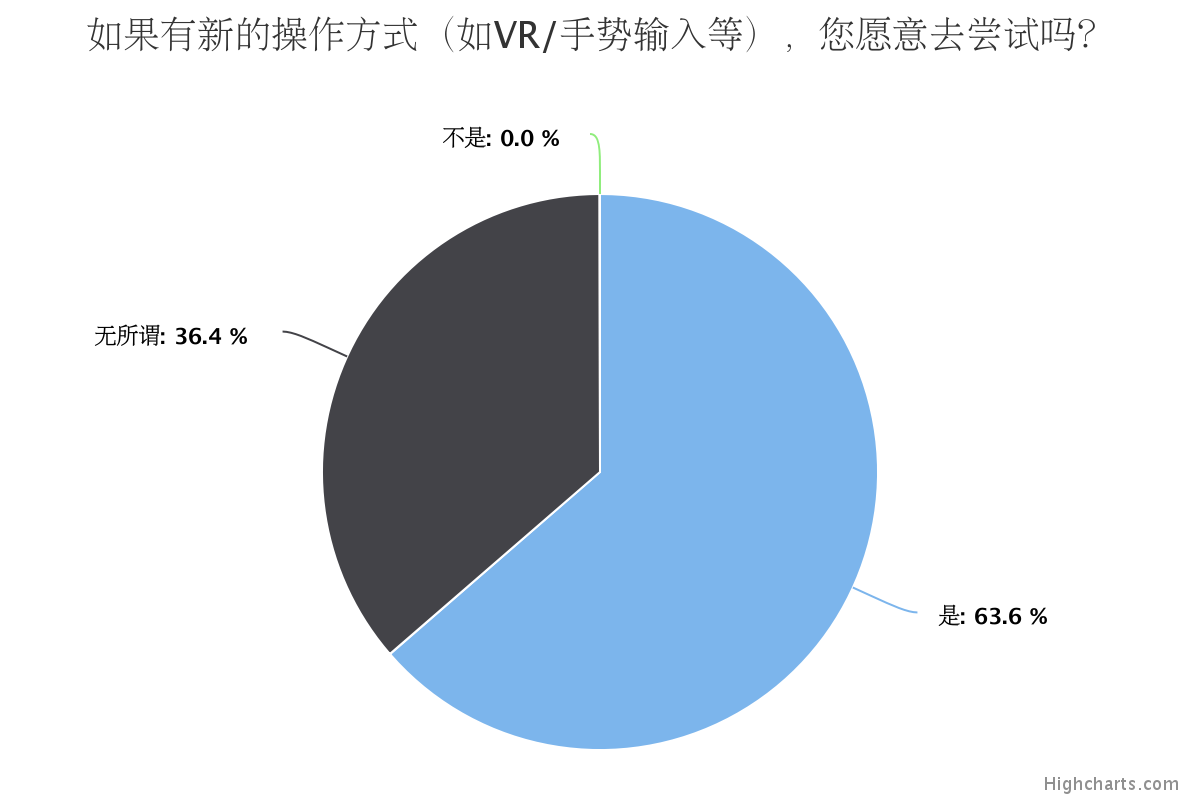
\includegraphics[width=20em]{chart3.png}\\
  \caption{}\label{2-3}
\end{minipage}
\begin{minipage}{0.5\linewidth}
  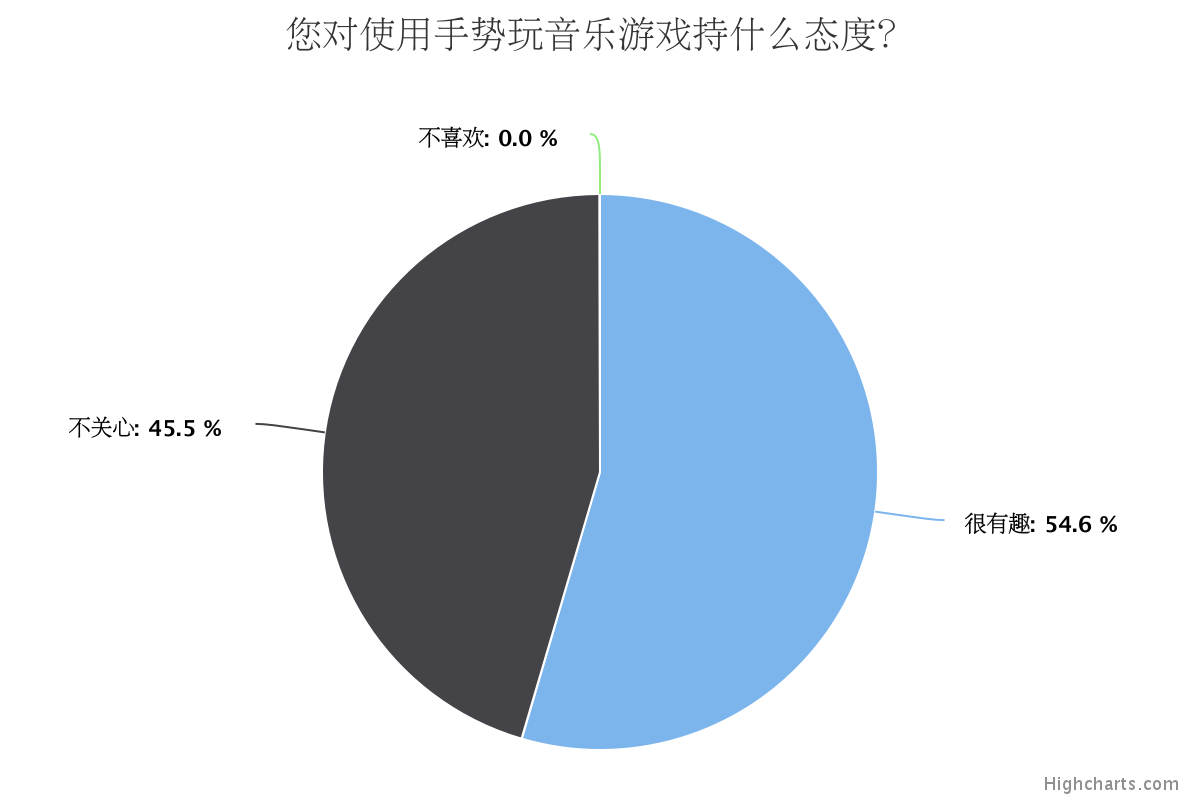
\includegraphics[width=20em]{chart4.png}\\
  \caption{}\label{2-4}
\end{minipage}
\end{figure}
\paragraph{}
游戏玩家对于新鲜的事物总是投以最高的好奇和憧憬,特别是新的与游戏的交互模式,相信吸引到不少用户的眼球。但是新的交互方式也意味着新的缺陷,现在手势输入还未普及,大部分玩家没有LeapMotion等设备,
这也将是我们推广的一个限制。但是最近游戏厂商占领VR市场之风越演越烈,Sony、Vavle纷纷加入竞争,大力推广VR设备,相信不久的将来,VR/AR游戏将会是游戏市场的一大发展方向,也会有更多的人进入VR的世界,进行游戏。
所以Cubeat也顺应了游戏市场的方向。
\paragraph{是否愿意尝试Cubeat类的游戏}
\paragraph{}
个人认为游戏的实际效果需要玩过才能知道,不易描述,所以本调查结果仅供参考
\begin{figure}[H]
  \centering
  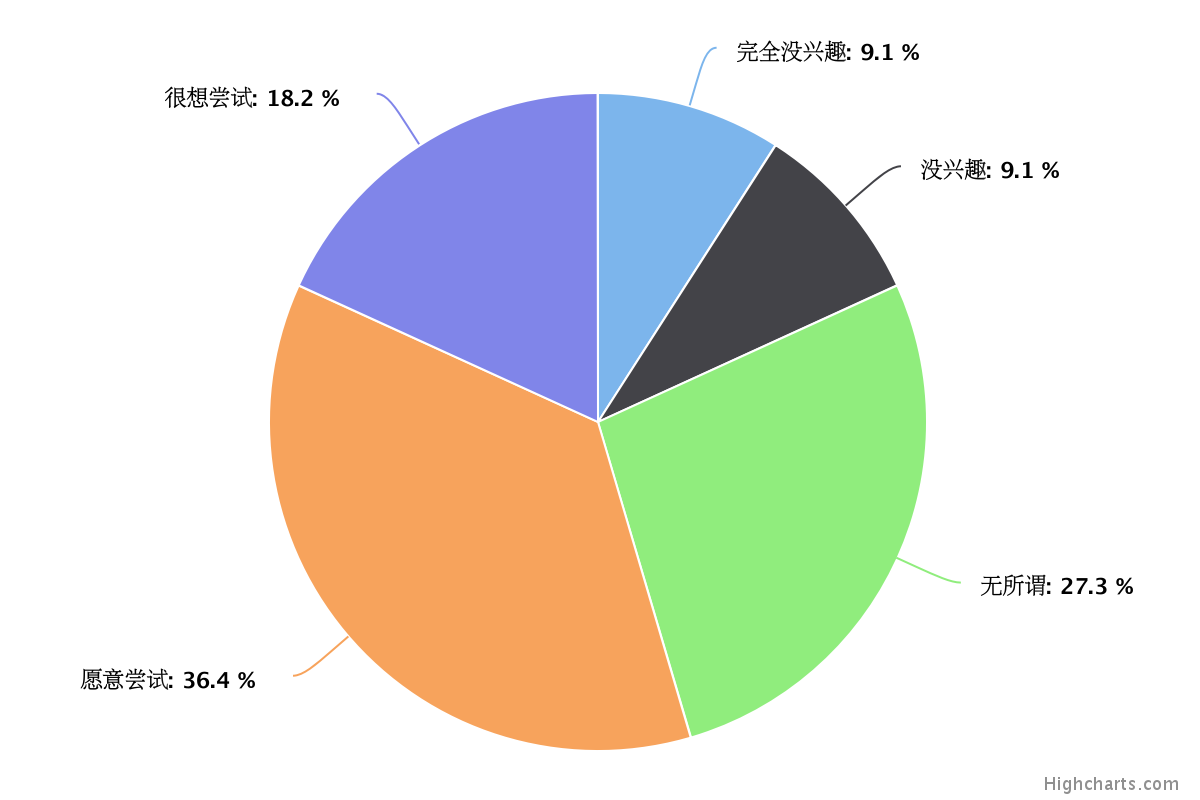
\includegraphics[width=22em]{chart5.png}\\
  \caption{是否愿意尝试以模仿作为载体手势输入的音乐游戏}\label{2-5}
\end{figure}
\paragraph{}
总之,调查结果出乎我们的意料。以往我们以为音乐游戏受众群体较小,但实际上年轻人中有许多人在玩音乐游戏。只是音乐游戏由于它自身的特性,很难获得精英玩家,导致许多玩家没有把主要精力放在音游上,而只是把它当做半个“音乐播放器”使用。
\paragraph{}
由于Cubeat输入方式的特性,我们游戏的可玩性将集中在玩法上,即使不愿意花费太多时间提高技术的玩家,也能从Cubeat中获得许多乐趣。
\subsection{同类产品}
\paragraph{}
分析完了用户,再从同类产品的角度分析一下Cubeat的可行性。在介绍同类产品之前,先介绍一下音游的几个基本概念
\begin{description}
  \item[铺面/难度] 在音乐游戏中,一首歌曲往往有多个难度,以供不同级别的玩家挑战。“铺面”或者“难度”一般就是指一首歌的某一个特定难度
  \item[note/物件] 一般指游戏中可供玩家击打的最小单位,一般对应音乐的一个音符或一个长音
  \item[BPM] beat per minutes 的缩写,乐曲的每分钟节拍数,用来衡量曲子的快慢。一般来说BPM越高的曲子,铺面越难
\end{description}
\paragraph{}
不同音乐游戏尽管画面不同,玩法不同,但是由于其以音乐为主体,总是逃不过这些概念和设计。
\paragraph{从“劲乐团”到“节奏大师”}
\paragraph{}
下落式(用按键或者触摸屏模拟弹钢琴)音乐游戏,作为音乐游戏的一大始祖,在PC还未流行时就已经在各大游戏机和街机上盛行。下落式非常精妙地设计了音乐游戏中音乐跟游戏连接的方式:使用钢琴键作为用户输入的接口,使用下落的音符作为音乐的接口。这种玩法一定程度上模拟了弹钢琴的动作,使得游戏简单直接容易让玩家上手。从十几年前的“劲乐团(O2jam)”到几年前的“节奏大师”、“deemo”等,均使用这个简单直观的设计,却都获得了很高的评价。
\begin{figure}[H]
\begin{minipage}{0.5\linewidth}
  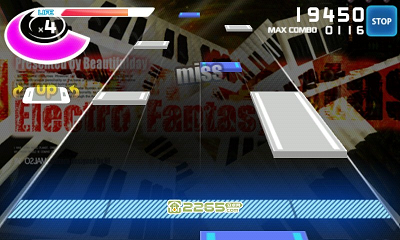
\includegraphics[width=15em]{O2jam.png}\\
  \caption{O2jam游戏截图}\label{3-1}
\end{minipage}
\begin{minipage}{0.5\linewidth}
  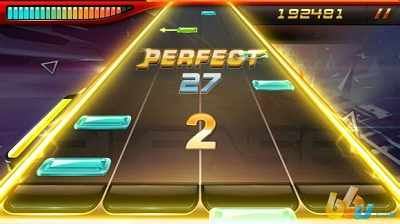
\includegraphics[width=15em]{rm.png}\\
  \caption{节奏大师游戏截图}\label{3-2}
\end{minipage}
\end{figure}
\paragraph{}
经历了十几年的发展,从最开始的玩家爆炸发展,到现在的审美疲劳,下落式音乐游戏已经渐渐走向衰落。从“劲乐团”到“节奏大师”,游戏模式没有变化,只是一个模子从PC被搬到了移动设备上来。
“劲乐团”早已关服停运,“节奏大师”玩家也不增反减,许多玩家抱怨下落式这种传统的游戏模式已经难以给自己带来乐趣。\\
\textbf{比较}
\begin{description}
  \item[玩法] 玩法陈旧缺乏创意,玩家慢慢审美疲劳
  \item[可玩性] 只有按键一种操作,较为单调
  \item[平台] 可以在PC/移动设备/街机上游戏,适用面较广
\end{description}
\paragraph{创新、变革}
音乐游戏是个大的话题,游戏制作者不会拘泥于一种玩法,许多标新立异的音乐游戏也是层出不穷。它们或是模拟除钢琴外其他乐器,或是用其他领域简单直观的东西代替琴键,成为玩家游戏的输入。下面举几个有代表性的这类作品
\paragraph{}
\textbf{乐动魔方}\\
乐动魔方是Konami公司出品的一款街机音乐游戏,后被移植到IOS和安卓平台。游戏方式十分简单,即在一个4X4的格子上会伴随音乐出现一些标示,玩家需要等待最佳时机点击标示,也就是音游圈俗称的“打地鼠”模式。
\paragraph{}
乐动魔方要求玩家在16个格子上精准点击,比较难的铺面甚至会同时出现5、6个note需要玩家点击。所以玩家一般都在街机或是平板上玩“乐动魔方”。另外,虽然它脱离了下落式的束缚,但是相对简单的画面和玩法
也容易让玩家审美疲劳。但是作为Konami公司的产品,众多的原创音乐支持了它健康地发展,并在音游市场站稳了脚步。
\textbf{比较}
\begin{description}
  \item[玩法] 较传统音游有所进步,但是输入方式仍有限制,需要在较大的屏幕甚至游戏厅的街机上玩。Cubeat则只需带一个小巧的LeapMotion即可
  \item[内容] 官方提供乐曲和乐谱,玩家可以根据官方乐曲自制乐谱,内容有限。Cubeat支持玩家自己输入乐曲自制铺面
\end{description}
\paragraph{}
\textbf{Lovelive!}\\
“Lovelive!”,大名鼎鼎的LL是音乐娱乐公司Lantis的一项大型企划中的音乐游戏,在多个平台有多个版本,这里主要介绍的是它在智能手机和平板上发售的版本。游戏本身玩法传承下落式,只不过用圆圈代替了方形的按键,并把水平的“钢琴”变为了一个半弧形。
\begin{figure}
  \centering
  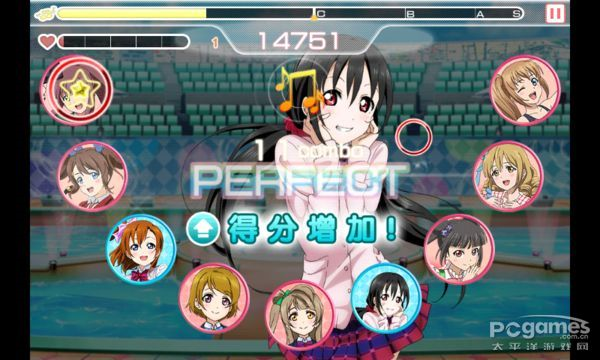
\includegraphics[width=24em]{ll.png}\\
  \caption{Lovelive!游戏画面}\label{3-3}
\end{figure}
\paragraph{}
Lovelive!作为较早将音乐游戏和手机游戏流行的“抽卡”、“活动”等元素结合起来的一款游戏,首先在日本获得了超高的人气。但是与其说它的成功是游戏模式

\paragraph{}
\section{目标}
做出有一定游戏性的通过识别手势进行输入的一个音乐游戏。作为一款音乐游戏,应该具有以下特性:
\begin{description}
  \item[完善的UI界面] 为用户提供基本的图形界面交互
  \item[丰富炫酷的游戏画面] 有一定的画面特效,用炫酷的画面给玩家更多积极的反馈
  \item[完整的游戏模式] 以音乐为背景,使玩家的操作需要契合节拍
\end{description}
\paragraph{}
除此之外,我们还有以下较其他音乐游戏创新的功能
\begin{itemize}
  \item 自带编辑器功能,让玩家也能轻松参与到编铺中来,方便构成玩家社区
  \item 多种基本手势输入法,比如手指点击,滑动,手掌翻动等
  \item
\end{itemize}

\section{创新点}
使用手势操作,革新了传统音乐游戏的玩法。
\section{技术支持}
\begin{itemize}
  \item Leap Motion硬件支持
  \item 手势识别
  \item 游戏设计方法
\end{itemize}
\end{document}
